\section{Zielsetzung}
Ziel des Versuches ist es die Brennweite $f$ von verschiedenen Linsen mit zwei Methoden zu bestimmen. Dazu wird zunächst das Abbildungsgesetz und die Linsengleichung verifiziert. Zusätzlich wird die chromatische Abberation untersucht.

\section{Theoretische Grundlage}
\begin{minipage}[T]{0.5\textwidth}
Im Allgemeinen werden Linsen aus einem Material gefertigt, welches einen anderen Brechungsindex aufweist, als die umgebende Luft. Durch den unterschiedlichen Brechungsindex wird das eintreffende Licht, nach dem Brechungsgesetz, gebrochen. Die Linsen werden in zwei Gruppen eingeteilt: die Sammellinsen und die Zerstreuungslinsen. Die Sammellinsen werden zum Linsenrand dünner, wodurch parralleles Licht im Brennpunkt gebündelt wird. Bei Sammellinsen sind die Brennweite $f$ und die Bildweite $b$ immer positiv und es entsteht ein reelles Bild. Im Gegensatz dazu wird die Zerstreuungslinse zum Linsenrand hin breiter. Außerdem sind Brennweite $f$ und Bildweite $b$ negativ. Das entstehende Bild wird als virtuell bezeichnet. Die Abbildung (\ref{fig:Bild1}) zeigt die Bildkonstruktion von einer dünnen Sammellinse (Oben), einer dünnen Zerstreuungslinse (Mitte) und einer dicken Sammellinse (Unten). Bei dünnen Linsen wird die Brechung auf die Mittelebene der Linse reduziert. Dies ist bei dicken Linsen nicht mehr möglich und es werden zwei Hauptebenen eingeführt an denen sich das Licht bricht. Zur Bildkonstrucktion werden drei ausgezeichnete Strahlen verwendet:
\end{minipage}
\begin{minipage}[T]{0.5\textwidth}
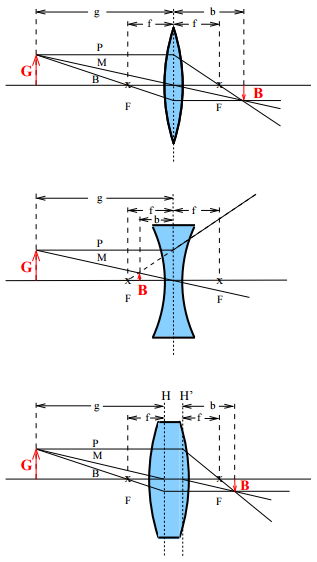
\includegraphics[width=1\textwidth]{picture/Bild1.PNG}
\label{fig:Bild1}
\end{minipage}
Der Parrallelstrahl $P$ läuft vom Gegenstand $G$ parrallel zur optischen Achse zur Linse und wird dort so gebrochen, dass er durch den Bildpunkt $B$ läuft. \\
Der Mittelpunktsstrahl läuft vom Gegenstand $G$ direkt zum Bildpunkt $B$ ohne durch die Linse gebrochen zu werden.\\
Der Brennpunktstrahl läuft vom Gegenstand $G$ zur Linse und wird dort so gebrochen, dass er danach parrallel zur optischen Achse läuft und die beiden anderen Strahlen im Bildpunkt $B$ schneidet.
\newpage

Mithilfe der Strahlensätze lässt sich das Abbildungsgesetz, an den Fällen in \\ Abbildung (\ref{fig:Bild1}), herleiten:
\begin{equation}
	V = \frac{B}{G} = \frac{b}{g} \ .
	\label{eqn:V}
\end{equation}
$B$ und $G$ entprechen der Bild- bzw. Gegenstandsgröße und $b$ und $g$ der Bild- bzw. Gegenstandweite. Für dünne Linsen folgt aus dem Abbildungsgesetz und der Bildkonstruktion die Linsengleichung:
\begin{equation}
	\frac{1}{f} = \frac{1}{b} + \frac{1}{g} \ .
	\label{eqn:D}
\end{equation}
Bei dicken Linsen und Linsensystemen wird nun die Mittelebene durch zwei Hauptebenen $H$ und $H'$ ersetzt an denen die Strahlen gebrochen werden. Die Brennweite, die Gegenstandsweite und die Bildweite werden zu der jeweiligen Hauptebene bestimmt, dadurch behält die Linsengleichung ihre Gültigkeit. Die Vereinfachung der Brechung an der Mittelebene bzw. der Hauptebenen nur für achsennahe Strahlen, da bei achsenfernen Strahlen das Licht stärker gebrochen wird. Bei der sphärischen Abberration liegt der Brennpunkt von achsennahen Strahlen weiter weg von der Linse als bei achsenfernen Strahlen. Durch dieses Phänomen wird das Bild unscharf, dies kann allerdings durch eine Irisblene, welche die achsenfernen Strahlen ausblendet, gelöst werden. \\
Außerdem muss beachtet werden, dass der Brechungsindex von der Wellenlänge, des einfallenden Lichtes, abhängt. Dadurch entsteht die chromatische Abberration. Das heißt blaues Licht wird stärker gebrochen als rotes Licht.

\subsection{Bestimmung der Brennweite einer Linse nach Bessel}
Dafür wird der Abstand $e$ und der Abstand $d$ konstant gehalten (siehe Abbildung (\ref{fig:Bessel})).
\begin{figure}[H]
	\centering
	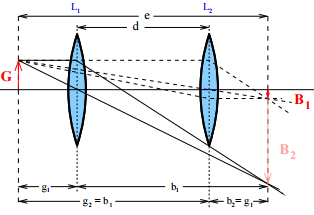
\includegraphics[height=5cm]{picture/Bessel}
	\caption{Schematische Darstellung für die Methode von Bessel.}
	\label{fig:Bessel}
\end{figure}
Der Abstand $e$ ist gleich
\begin{align*}
	e = g_1 + b_1 = g_2 + b_2
\end{align*}
und $d$ entspricht
\begin{align*}
	d = g_1 - b_1 = g_2 - b_2 \ .
\end{align*}
Durch einsetzen läßt sich die Brennweite der Linse zu
\begin{equation}
	f = \frac{e^2 - d^2}{4e}
	\label{eqn:tbes}
\end{equation}
bestimmen.

\subsection{Bestimmung der Brennweite eines Linsensystems nach Abbe}
Dafür muss neben der Brennweite $f$, auch die Lage der beiden Hauptebenen $H$ und $H'$ ermittelt werden. Dies geschieht über das Abbildungsgesetz (siehe Gl. (\ref{eqn:V})). Wie in Abbildung (\ref{fig:Abbe}) zu erkennen ist, werden dazu die Bild- und Gegenstandsweiten $g'$ und $b'$ bezüglich eines beliebigen Punktes $A$ gemessen. Aus den Formeln
\begin{equation}
	g' = g + h = f \cdot \left( 1 + \frac{1}{V} \right) + h
	\label{eqn:g'}
\end{equation}
und
\begin{equation}
	b' = b + h' = f \cdot (1 + V) + h'
	\label{eqn:b'}
\end{equation}
ergeben sich dann die Brennweite $f$ und die Lage der Hauptebenen.

\begin{figure}[H]
	\centering
	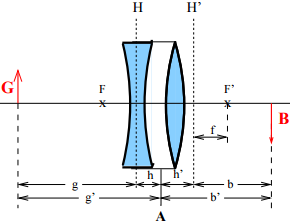
\includegraphics[height=5cm]{picture/Abbe}
	\caption{Schematische Darstellung für die Methode von Abbe.}
	\label{fig:Abbe}
\end{figure}
